%%%%%%%%%%%%%%%%%%%%%%%%%%%%%%%%%%%%%%%%%%%%%%%%%%%%%%%%%%%%%%5
%% ITB Author: Markus Hofmann - markus.hofmann@itb.ie
%% Adapted from Dalhousie University
%%%%%%%%%%%%%%%%%%%%%%%%%%%%%%%%%%%%%%%%%%%%%%%%%%%%%%%%%%%%%%%5


\documentclass[12pt,ITBthesis]{report}

\usepackage{amsfonts}
\usepackage{amssymb,amsmath}
\usepackage{amsthm}
\usepackage{newlfont}
\usepackage{graphicx}
\usepackage{tabularx}
\usepackage{longtable}
\usepackage{lscape}
%\usepackage{rotating}
\usepackage{latexsym}
\usepackage{natbib}
\usepackage{geometry}
\usepackage{fancyhdr}
\usepackage{xthesis}
\usepackage{xtocinc} %Include Table of Contents as the first entry in TOC
\usepackage{subfigure}
\usepackage{times}
\usepackage[hidelinks]{hyperref}

\bibpunct[, ]{(}{)}{;}{a}{,}{,}


\begin{document}

%%% this section is responsible for creating bookmarks and cross-links in your pdf document
%\hypersetup{bookmarksnumbered=true, colorlinks=false, bookmarksopen = false, linkcolor=blue ,
%linkbordercolor = 3 3 3, citebordercolor = 3 3 3, urlbordercolor = 3 3 3}


% Fuzz -------------------------------------------------------------------
\hfuzz2pt % Don't bother to report over-full boxes if over-edge is < 2pt
% Line spacing -----------------------------------------------------------

\newlength{\defbaselineskip}
\setlength{\defbaselineskip}{\baselineskip}
\newcommand{\setlinespacing}[1]%
           {\setlength{\baselineskip}{#1 \defbaselineskip}}
\newcommand{\doublespacing}{\setlength{\baselineskip}%
                           {2.0 \defbaselineskip}}
\newcommand{\singlespacing}{\setlength{\baselineskip}{\defbaselineskip}}
% MATH -------------------------------------------------------------------
\newcommand{\A}{{\cal A}}
\newcommand{\h}{{\cal H}}
\newcommand{\s}{{\cal S}}
\newcommand{\W}{{\cal W}}
\newcommand{\BH}{\mathbf B(\cal H)}
\newcommand{\KH}{\cal  K(\cal H)}
\newcommand{\Real}{\mathbb R}
\newcommand{\Complex}{\mathbb C}
\newcommand{\Field}{\mathbb F}
\newcommand{\RPlus}{[0,\infty)}
%
\newcommand{\norm}[1]{\left\Vert#1\right\Vert}
\newcommand{\essnorm}[1]{\norm{#1}_{\text{\rm\normalshape ess}}}
\newcommand{\abs}[1]{\left\vert#1\right\vert}
\newcommand{\set}[1]{\left\{#1\right\}}
\newcommand{\seq}[1]{\left<#1\right>}
\newcommand{\eps}{\varepsilon}
\newcommand{\To}{\longrightarrow}
\newcommand{\RE}{\operatorname{Re}}
\newcommand{\IM}{\operatorname{Im}}
\newcommand{\Poly}{{\cal{P}}(E)}
\newcommand{\EssD}{{\cal{D}}}
% THEOREMS ---------------------------------------------------------------
\theoremstyle{plain}
\newtheorem{thm}{Theorem}[section]
\newtheorem{cor}[thm]{Corollary}
\newtheorem{lem}[thm]{Lemma}
\newtheorem{prop}[thm]{Proposition}
%
\theoremstyle{definition}
\newtheorem{defn}{Definition}[section]
%
\theoremstyle{remark}
\newtheorem{rem}{Remark}[section]
%
\numberwithin{equation}{section}
\renewcommand{\theequation}{\thesection.\arabic{equation}}
%%% ----------------------------------------------------------------------
\setlength{\tclineskip}{1.05\baselineskip}
%%% ----------------------------------------------------------------------
\makeatletter
\renewcommand\appendix{%
 \par
 \setcounter{chapter}{0}%
 \setcounter{section}{0}%
 \setcounter{subsection}{0}%
 \gdef\thesection{\@Alph\c@section}
 \gdef\@sect##1##2##3##4##5##6[##7]##8{%
  \refstepcounter{##1}%
  \protected@edef\@svsec{\@seccntformat{##1}\relax}%
  \begingroup
    \hspace{-\parindent}##6\appendixname~ {%
    \@hangfrom{\hskip ##3 \relax\@svsec}\par%
    \hspace{-\parindent}\interlinepenalty \@M ##8 \@@par}%
  \endgroup
  \csname ##1mark\endcsname{##7}%
  \addcontentsline{toc}{##1}{\protect\numberline{\csname the##1\endcsname}##7}%
  \@xsect{##5}%
 }%
}%
\makeatother

\setlength{\parskip}{1ex plus 0.5ex minus 0.2ex}


\title{Utilisation of Electronic Fare Collection data of Urban Bus Operators with regard to Transfer
Journeys and Origin/Destination Estimation}

\author{Markus Hofmann }

\university{Institute of Technology Blanchardstown }

\dept{School of Informatics and Engineering }

\address{Dublin, Ireland }

\supervisor{Dr. Simon Wilson, Prof. Peter White }

\submitdate{10 October 2005 }

\degree{M.Sc. in Computing }


%\dedicate{To my wife\\
% \begin{Huge}{\textbf{Glenda}}\end{Huge}}

%\nobib
%\draft
%\nofront
%\permissionfalse
%\include{ABS}

\setcounter{page}{1} \beforepreface



{ \typeout{Abbreviations}
% Thesis Abbreviation ------------------------------------------------------

\prefacesection{Abbreviations}


%%%%%%%%%%%%%%%%%%%%%%%%%%%%%%%%%%%%%%%%%%%%%%%%%%%%%%%%%%%%%%%%%%%%%%%%%%%%%%%%
% Create a list of all abbreviations that you've used throughout your thesis.  %
% Order the abbreviations in alphabetical order                                %
%%%%%%%%%%%%%%%%%%%%%%%%%%%%%%%%%%%%%%%%%%%%%%%%%%%%%%%%%%%%%%%%%%%%%%%%%%%%%%%%

\begin{longtable}{p{90pt}l}
\hline ADA      & Americans Disability Act \\
\hline AVAS     & Automated Voice Annunciation System \\
\hline AVL      & Automatic Vehicle Location \\
\hline CBD      & Central Business District \\
\hline CBR      & Case-Based Reasoning \\
\hline CIE      & C\'{o}ras Iompair \'{E}ireann \\
\hline CTA      & Chicago Transport Authority \\
\hline DD       & Double Decks \\



\hline
\end{longtable}






% ----------------------------------------------------------------------
 %write your list of abbreviations in a file called abbreviations.tex
}

%{ \typeout{Glossary}
%\include{glossary}
%}



% ------------------------------------------------------------------------
\afterpreface
\def\baselinestretch{1}
\setlinespacing{1.66}
% ------------------------------------------------------------------------

\pagestyle{fancy}
\renewcommand{\chaptermark}[1]%
{\markboth{\MakeUppercase{\thechapter.\ #1}}{}}
\renewcommand{\sectionmark}[1]%
{\markright{\MakeUppercase{\thesection.\ #1}}}
\renewcommand{\headrulewidth}{0.5pt}
\renewcommand{\footrulewidth}{0pt}
\newcommand{\helv}
{%
\fontfamily{bch}\fontseries{b}\fontsize{9}{11}\selectfont} \fancyhf{} \fancyhead[LE,RO]{\helv \thepage}
\fancyhead[LO]{\helv \rightmark} \fancyhead[RE]{\helv \leftmark}

% ------------------------------------------------------------------------
\setlinespacing{1.0}

\setlinespacing{1.1}


\chapter{Introduction and Background} \label{sec:introduction}

\section{section header 1}

\subsection{Subsection header 1}
fdsdfsdfds
\subsection{Subsection header 2}
fdsdfsdfds
\subsection{Subsection header 3}
fdsdfsdfds


\section{section header 2}

\subsection{Subsection header 1}

Figure \ref{Figure: Map of the Greater Dublin Area} shows a spatial map of the GDA.

\begin{figure}[htbp]
\center 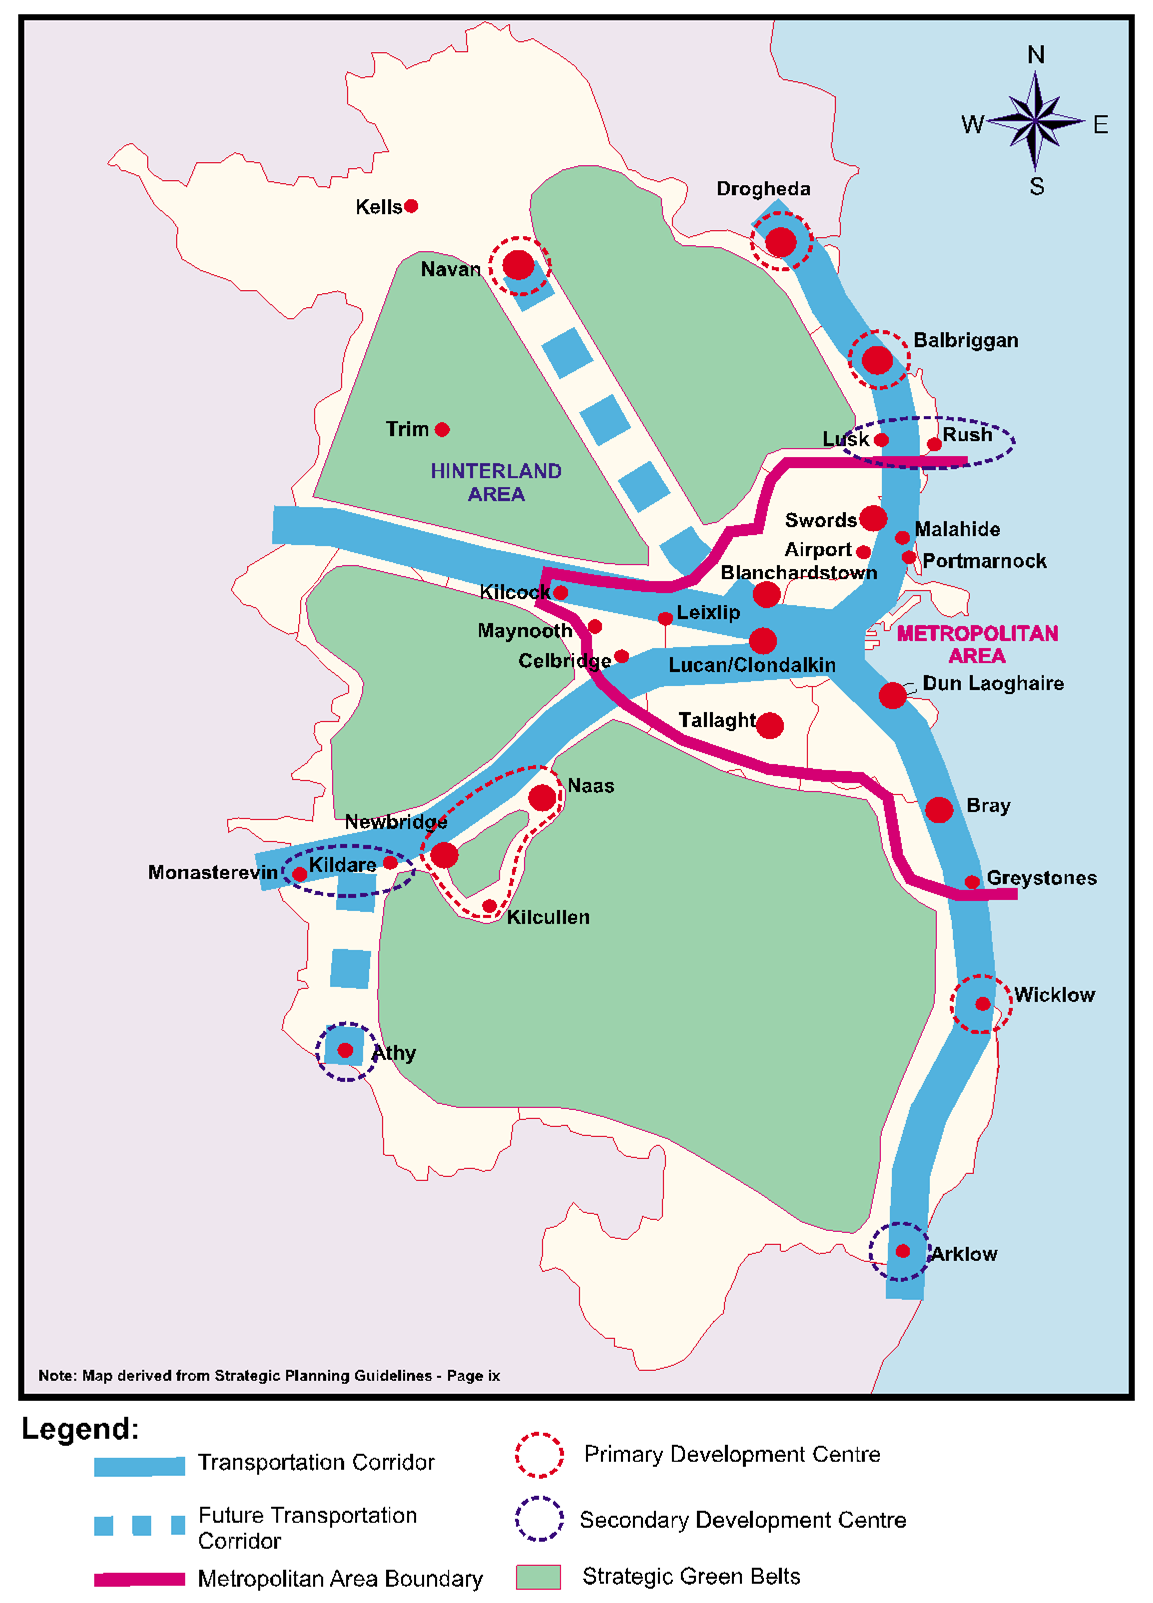
\includegraphics[width=400pt]{intro1}\\
\caption{Map of the Greater Dublin Area \citep{PLA01}} \label{Figure: Map of the Greater Dublin
Area}
\end{figure}

\newpage

\begin{table}[htbp]
\footnotesize{} \setlinespacing{1.0} \vspace{10pt} \begin{longtable} {p{190pt}cccc}
\caption{Demographic Projections of the GDA} \\
\hline

\textbf{Greater Dublin Area}&

\textbf{1991}  & \textbf{1996}& \textbf{1999}& \textbf{2016} \\* \hline \hline {Population
(million) }&

{1.35}  & {1.41}& {1.46}& {1.75} \\* \hline {Households ('000) }&

{402}  & {446}& {521}& {675} \\* \hline {Employment ('000) }&

{452}  & {549}& {681}& {878} \\* \hline {Unemployment rate }&

{16{\%}}  & {12{\%}}& {6{\%}}& {5{\%}} \\* \hline {Car Ownership (per 1000 population)}&

{247}  & {292}& {342}& {480} \\* \hline {{\%} Growth in GDP since 1991}& {- }& {42{\%}}& {79{\%}}&
{260{\%} }\\* \hline

\label{Table: Demographic Projections of the GDA}
\end{longtable}
 \normalsize{} \setlinespacing{1.1}
\end{table}

\newpage

\begin{figure}[htbp]
\center 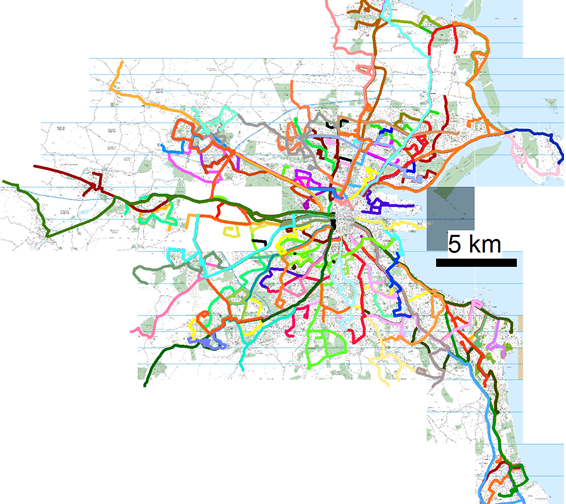
\includegraphics[width=400pt]{intro2}\\
\caption{Map of Bus Routes of Dublin Bus} \label{fig2: Map of bus routes provided by Dublin Bus}
\end{figure}

The figures shown in Table \ref{Table: Demographic Projections of the GDA} are taken from the
website of Dublin Bus \citep{DUB05}. The bus fleet is broken down into depot location and bus
category.

\subsection{Subsection header 2}
fdsdfsdfds
\subsection{Subsection header 3}
fdsdfsdfds

\section{section header 3}

\subsection{Subsection header 1}
fdsdfsdfds
\subsection{Subsection header 2}
fdsdfsdfds
\subsection{Subsection header 3}
fdsdfsdfds

\section{section header 4}

\subsection{Subsection header 1}

Latex is very good when mathematical formulas need to be displayed:

\begin{equation}\label{taeq2}
    S_{ij}=1-{\frac{|(F_{ij}-F^T_{ij})|}{(F_{ij}+F^T_{ij})}}
\end{equation}


\subsection{Subsection header 2}
\subsection{Subsection header 3}

\chapter{Literature Review}


\section{section header 1}

\subsection{Subsection header 1}
fdsdfsdfds
\subsection{Subsection header 2}
fdsdfsdfds
\subsection{Subsection header 3}
fdsdfsdfds


\section{section header 2}

\subsection{Subsection header 1}
fdsdfsdfds
\subsection{Subsection header 2}
fdsdfsdfds
\subsection{Subsection header 3}
fdsdfsdfds

\section{section header 3}

\subsection{Subsection header 1}
fdsdfsdfds
\subsection{Subsection header 2}
fdsdfsdfds
\subsection{Subsection header 3}
fdsdfsdfds

\section{section header 4}

\subsection{Subsection header 1}
\subsection{Subsection header 2}
\subsection{Subsection header 3}

\chapter{Methodology Chapter}


\section{section header 1}

\subsection{Subsection header 1}
fdsdfsdfds
\subsection{Subsection header 2}
fdsdfsdfds
\subsection{Subsection header 3}
fdsdfsdfds


\section{section header 2}

\subsection{Subsection header 1}
fdsdfsdfds
\subsection{Subsection header 2}
fdsdfsdfds
\subsection{Subsection header 3}
fdsdfsdfds

\section{section header 3}

\subsection{Subsection header 1}
fdsdfsdfds
\subsection{Subsection header 2}
fdsdfsdfds
\subsection{Subsection header 3}
fdsdfsdfds

\section{section header 4}

\subsection{Subsection header 1}
\subsection{Subsection header 2}
\subsection{Subsection header 3}

%\include{chapter4}
%\include{chapter5}
%\include{chapter6}
%\include{chapter7}
%\include{chapter8}





\setlinespacing{1.0}
\bibliographystyle{plainnat}
\bibliography{bibliography}

\appendix
%\chapter*{Appendices}
   \nonumchapter{Appendices}

\newpage

\section{Structure of Dublin Bus Wayfarer Data }
\label{app:structure} \textbf{Introduction}

Dublin Bus uses electronic fareboxes

\newpage



\section{Coarse Zone Description}
\label{Appendix: Coarse Zone Description}


\begin{longtable}
{cl} \hline
\endhead
\hline
\endfoot
\textbf{{Coarse Zone}}&
\textbf{{Coarse Zone Description}} \\
\hline \hline\textbf{{1}}&
{City Centre (within Canal Ring)} \\
\hline \textbf{{2}}&
{Dublin Port Area} \\
\hline \textbf{{3}}&
{North East City (Clontarf, Raheny, Ayrfield)} \\
\hline \textbf{{4}}&
{North West City (Cabra, Finglas, Ballymun)} \\
\hline \textbf{{5}}&
{South East City (Rathmines)} \\
\hline \textbf{{6}}&
{South West City (Kilmainham, Walkingstown, Kimmage)} \\
\hline \textbf{{7}}&
{Fingal West (Blanchardstown / Castleknock)} \\
\hline \textbf{{8}}&
{Fingal East (Portmarnock, Malahide, Donabate, Swords, Airport)} \\
\hline \textbf{{9}}&
{Fingal North West (Naul, Ballyboghill, Oldtown)} \\
\hline \textbf{{10}}&
{Fingal North East (Rush, Lusk, Skerries, Balbriggan)} \\
\hline \textbf{{11}}&
{South Dublin - Lucan, Clondalkin} \\
\hline \textbf{{12}}&
{South Dublin - Tallaght} \\
\hline \textbf{{13}}&
{South Dublin - Saggart, Rathcoole, Bohernabrena} \\
\hline \textbf{{14}}&
{Dun Laogharie / Rathdown - North} \\
\hline \textbf{{15}}&
{Dun Laoghaire / Rathdown - South} \\
\hline \textbf{{16}}&
{Meath} \\
\hline \textbf{{17}}&
{Kildare} \\
\hline \textbf{{18}}&
{West Wicklow} \\
\hline \textbf{{19}}&
{East Wicklow} \\
\hline \textbf{{20}}&
{Louth} \\
\hline \textbf{{21}}& {Externals} \label{tab1}
\end{longtable}

\newpage

\section{Coarse Zone Map}
\label{Appendix:Coarse Zone Map}


%\begin{figure}[hbtp]
%\center
%  % Requires \usepackage{graphicx}
%  \includegraphics[width=327pt]{dtomap}\\
%
%\end{figure}

\newpage








\section{Ticket Types}\label{app:tickettypes}
\footnotesize{} \setlinespacing{1.0}
\begin{longtable}[htbp]
{cc} \hline \textbf{Ticket Type ID} & \textbf{Description} \\\hline \hline \hline
\endhead

 300&
Feeder Ticket - Child \\
\hline 301&
Feeder Ticket - Adult \\
\hline 310&
10-Journey Feeder - Adult \\
\hline 317&
Airlink Adult Airport-Busarus \\
\hline 318&
Airlink Child Airport-Busarus \\
\hline 319&
Airlink Child Airport-Heuston \\
\hline 320&
Airlink Adult Airport-Heuston \\
\hline 333&
Adult Single Feeder \\
\hline 365&
Child Bus/Rail Short Hop - Day \\
\hline 366&
Adult Bus/Rail Short Hop - Day \\
\hline 367&
Family Bus/Rail Short Hop - Day \\
\hline 369&
4 Day Explorer \\
\hline 410&
Weekly Adult Short Hop Bus/Rail \\
\hline 430&
Weekly Adult Medium Hop Bus/Rail \\
\hline 431&
Weekly Adult Long Hop Bus/Rail \\
\hline 432&
Weekly Adult Giant Hop Bus/Rail \\
\hline 433&
Monthly Adult Short Hop Bus/Rail \\
\hline 455&
Monthly Adult Long Hop Bus/Rail \\
\hline 456&
Monthly Adult Giant Hop Bus/Rail \\
\hline 457&
Monthly Student Short Hop Bus/Rail \\
\hline 458&
Annual Bus/Rail \\
\hline 478&
Annual All CIE Services \\
\hline 479&
Annual CIE Pensioner Bus/Rail \\
\hline 480&
Monthly CIE Pensioner Bus/Rail \\
\hline 493&
Foreign Student - 1 Week \\
\hline 494&
Foreign Student - 2 Week \\
\hline 495&
Foreign Student - 3 Week \\
\hline 496&
Foreign Student - 4 Week \\
\hline 497&
CYC Group \\
\hline 600&
Adult Cash Fare \\
\hline 608&
Nitelink (Maynouth/Celbridge) \\
\hline 609&
Nitelink (Maynouth/Celbridge) \\
\hline 610&
Child Cash Fare \\
\hline 620&
Schoolchild Cash Fare \\
\hline 625&
Adult (formerly Shopper) \\
\hline 630&
Adult 10-Journey (3 Stages) \\
\hline 631&
Adult 10-Journey (7 Stages) \\
\hline 632&
Adult 10-Journey (12 Stages) \\
\hline 633&
Adult 10-Journey (23 Stages) \\
\hline 634&
Adult 10-Journey (23+ Stages) \\
\hline 640&
Adult 2-Journey (3 Stages) \\
\hline 641&
Adult 2-Journey (7 Stages) \\
\hline 642&
Adult 2-Journey (12 Stages) \\
\hline 643&
Adult 2-Journey (23 Stages) \\
\hline 644&
Adult 2-Journey (23+ Stages) \\
\hline 650&
Schoolchild 10-Journey \\
\hline 651&
Scholar 10-Journey \\
\hline 652&
Schoolchild 2-Journey \\
\hline 653&
Scholar 2-Journey \\
\hline 657&
Transfer 90 (or Passenger Change) \\
\hline 658&
Adult Single Heuston-CC \\
\hline 660&
Adult One Day Travelwide \\
\hline 661&
Child One Day Travelwide \\
\hline 662&
Family One Day Travelwide \\
\hline 665&
Rambler (3 Day Bus only) \\
\hline 670&
Weekly Adult Bus \\
\hline 671&
Weekly Adult Cityzone \\
\hline 690&
Weekly Student Travelwide \\
\hline 691&
Weekly Student Cityzone \\
\hline 705&
Monthly Adult Citizone (AerLingus.) \\
\hline 710&
Monthly Adult Travelwide \\
\hline 730&
Annual Adult Travelwide \\
\hline 760&
Annual Staff Bus \\
\hline 790&
School Pass \\
\hline 791&
OAP Pass \\
\hline 800&
City Tour - Adult \\
\hline 801&
City Tour - Family \\
\hline 802&
City Tour - Child \\
\hline 898& 10 - Journey Test Ticket \\\hline \label{tab1}
\end{longtable}
 \normalsize{} \setlinespacing{1.1}

\newpage




\section{Ticket 1 -- 730-243}
\label{Appendix: Ticket 1 -- 730-243}

\footnotesize{} \setlinespacing{1.0} \vspace{10pt}

\begin{longtable}[htbp] {ccccccc} \hline
\textbf{Date}& \textbf{Stage}& \textbf{Boarding Time}&

\textbf{Route}   & \textbf{Direction}& \textbf{Zone}&
\textbf{Area} \\
\hline \hline 01/10/1999& 62& 08:03&

150   & 1& 12&
Templeogue \\
\hline 01/10/1999& 25& 18:26&

150   & 0& 1&
City Centre South \\
\hline 02/10/1999& 70& 10:03&

16   & 1& 6&
Harolds Cross \\
\hline 02/10/1999& 25& 14:38&

16   & 0& 1&
City Centre North \\
\hline 04/10/1999& 62& 08:29&

150   & 1& 12&
Templeogue \\
\hline 04/10/1999& 25& 18:37&

150   & 0& 1&
City Centre South \\
\hline 05/10/1999& 62& 08:07&

150   & 1& 12&
Templeogue \\
\hline 05/10/1999& 25& 17:21&

150   & 0& 1&
City Centre South \\
\hline 06/10/1999& 62& 07:49&

150   & 1& 12&
Templeogue \\
\hline 06/10/1999& 25& 17:25&

150   & 0& 1&
City Centre South \\
\hline 08/10/1999& 62& 08:12&

150   & 1& 12&
Templeogue \\
\hline 08/10/1999& 25& 18:13&

150   & 0& 1&
City Centre South \\
\hline 11/10/1999& 62& 08:37&

150   & 1& 12&
Templeogue \\
\hline 11/10/1999& 25& 18:12&

150   & 0& 1&
City Centre South \\
\hline 12/10/1999& 62& 07:27&

150   & 1& 12&
Templeogue \\
\hline 12/10/1999& 25& 14:47&

150   & 0& 1&
City Centre South \\
\hline 13/10/1999& 62& 08:17&

150   & 1& 12&
Templeogue \\
\hline 13/10/1999& 25& 13:34&

150   & 0& 1&
City Centre South \\
\hline 16/10/1999& 70& 08:07&

65B   & 1& 5&
Rathmines \\
\hline 16/10/1999& 25& 12:47&

16   & 0& 1&
City Centre North \\
\hline 19/10/1999& 62& 08:10&

150   & 1& 12&
Templeogue \\
\hline 19/10/1999& 25& 16:28&

150   & 0& 1&
City Centre South \\
\hline 20/10/1999& 62& 08:13&

150   & 1& 12&
Templeogue \\
\hline 20/10/1999& 25& 18:22&

150   & 0& 1&
City Centre South \\
\hline 21/10/1999& 62& 08:09&

150   & 1& 12&
Templeogue \\
\hline 21/10/1999& 25& 16:17&

150   & 0& 1&
City Centre South \\
\hline 22/10/1999& 62& 08:14&

150   & 1& 12&
Templeogue \\
\hline 22/10/1999& 25& 17:45&

150   & 0& 1&
City Centre South \\
\hline 27/10/1999& 62& 08:11&

150   & 1& 12&
Templeogue \\
\hline 27/10/1999& 25& 17:36&

150   & 0& 1&
City Centre South \\
\hline 28/10/1999& 62& 08:18&

150   & 1& 12&
Templeogue \\
\hline 28/10/1999& 25& 17:47&

150   & 0& 1&
City Centre South \\
\hline 29/10/1999& 62& 08:00&

150   & 1& 12&
Templeogue \\
\hline 29/10/1999& 25& 18:07&

150   & 0& 1&
City Centre South \\
\hline 30/10/1999& 70& 09:15&

16A   & 1& 6&
Harolds Cross \\
\hline 30/10/1999& 25& 14:53&

155   & 0& 0& City Centre South \\ \hline \label{tab14}
\end{longtable}
 \normalsize{} \setlinespacing{1.1}


\newpage


\section{Ticket 3 -- 730-73}
\label{Appendix: Ticket 3 -- 730-73}



\footnotesize{} \setlinespacing{1.0} \vspace{10pt}  \begin{longtable}[htbp] {ccccccc} \hline
\textbf{Date}& \textbf{Stage}& \textbf{Boarding Time}& \textbf{Route}& \textbf{Direction}&
\textbf{Zone}&
\textbf{Area} \\
\hline \hline 01/10/1999& 15& 07:45& 130& 1& 3&
Clontarf \\
\hline 01/10/1999& 75& 17:17& 130& 0& 1&
City Centre North \\
\hline 04/10/1999& 14& 07:49& 130& 1& 3&
Clontarf \\
\hline 04/10/1999& 75& 17:36& 130& 0& 1&
City Centre North \\
\hline 05/10/1999& 14& 07:55& 130& 1& 3&
Clontarf \\
\hline 05/10/1999& 75& 17:22& 130& 0& 1&
City Centre North \\
\hline 06/10/1999& 13& 07:42& 130& 1& 3&
Clontarf \\
\hline 06/10/1999& 75& 17:28& 130& 0& 1&
City Centre North \\
\hline 08/10/1999& 14& 07:56& 130& 1& 3&
Clontarf \\
\hline 08/10/1999& 75& 17:32& 130& 0& 1&
City Centre North \\
\hline 11/10/1999& 15& 07:43& 130& 1& 3&
Clontarf \\
\hline 11/10/1999& 75& 17:24& 130& 0& 1&
City Centre North \\
\hline 12/10/1999& 15& 07:53& 130& 1& 3&
Clontarf \\
\hline 12/10/1999& 75& 17:26& 130& 0& 1&
City Centre North \\
\hline 13/10/1999& 15& 07:53& 130& 1& 3&
Clontarf \\
\hline 13/10/1999& 75& 17:28& 130& 0& 1&
City Centre North \\
\hline 14/10/1999& 15& 07:58& 130& 1& 3&
Clontarf \\
\hline 14/10/1999& 75& 18:51& 130& 0& 1&
City Centre North \\
\hline 15/10/1999& 15& 07:53& 130& 1& 3&
Clontarf \\
\hline 15/10/1999& 75& 17:10& 130& 0& 1&
City Centre North \\
\hline 20/10/1999& 14& 07:46& 130& 1& 3&
Clontarf \\
\hline 20/10/1999& 75& 17:29& 130& 0& 1&
City Centre North \\
\hline 21/10/1999& 15& 08:07& 130& 1& 3&
Clontarf \\
\hline 21/10/1999& 75& 18:39& 130& 0& 1&
City Centre North \\
\hline 22/10/1999& 16& 08:07& 130& 1& 3&
Clontarf \\
\hline 22/10/1999& 75& 17:01& 130& 0& 1&
City Centre North \\
\hline 26/10/1999& 15& 07:51& 130& 1& 3&
Clontarf \\
\hline 26/10/1999& 75& 17:36& 130& 0& 1&
City Centre North \\
\hline 27/10/1999& 15& 07:52& 130& 1& 3&
Clontarf \\
\hline 27/10/1999& 75& 17:34& 130& 0& 1&
City Centre North \\
\hline 28/10/1999& 15& 08:09& 130& 1& 3&
Clontarf \\
\hline 28/10/1999& 75& 18:34& 130& 0& 1&
City Centre North \\
\hline 29/10/1999& 14& 07:59& 130& 1& 3&
Clontarf \\
\hline 29/10/1999& 75& 17:21& 130& 0& 1& City Centre North \\ \hline \label{tab16}
\end{longtable}
 \normalsize{} \setlinespacing{1.1}


\newpage




\end{document}
% ------------------------------------------------------------------------
%%%      \setlength\LTleft{1pt}
